\documentclass[Main]{subfiles}
\begin{document}

\chapter{Java Remote Method Invocation}
This chapter will cover the fundamentals in the distributed object-based system Java Remote Method Invocation (RMI) and how a leader of the distributed collaboration is elected.

\section{JAVA RMI}
Java Remote Method Invocation (RMI) is a middleware that supports Java-to-Java only. RMI gives a client on one Java Virtual Machine (JVM) access to objects that runs on another JMV which allows the client to invoke methods on the object - called the Remote Object. Thus providing remote communication between programs written in Java \cite{RMI-slides}. A JVM is a program that provides a run-time environment where applications written in Java binary code (called bytecode) can be executed. The JVM contains a set of instructions which is used when interpreting a Java bytecode enable the processor to execute a compiled Java program. The JVM will subsequently handle the actual execution of the program by interpreting each of its instructions, enabling automatic exception handling \cite[p. 422-423]{Tanenbaum}, \cite{wiki-jvm}.\\The remote object is a distributed object whose state always resides on one single JVM but whose interface can be made available to processes on another JVM \cite[p. 461]{Tanenbaum}.

\begin{figure}[H]
\centering
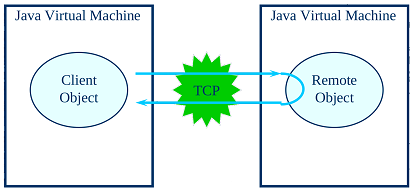
\includegraphics[scale=0.8]{Figurer/JVM.png}
\caption{System-overview of a Java RMI containing two JVM's \cite{RMI-slides}}
\label{Figure-jvm}
\end{figure}

The methods in the remote object can be accessed and invoked through an interface; the stub, which make the object appear as if it was a local object on the client's side. The interface is implemented as a proxy; a local representation of or placeholder for the remote object, which offers exactly the same interface as the remote object (the skeleton). The interface offers a declaration of the methods which can be invoked \cite[p. 461]{Tanenbaum}, \cite{RMI-slides}. During the communication between the two JVM's the complex data-structures which represents the object need to be transferred from one JVM to another. In order to facilitate this the object or its structures need to be serialized\footnote{The technique of serialization is typically called \textit{marshalling an object} in other programming languages than Java}; the data is translated into a format that can be transmitted across a network connection. The opposite operation; extracting a data-structure from a series of bytes is called deserialization \cite[p. 462]{Tanenbaum}, \cite{wiki-serialization}.

\subsection{The architecture and communication}
The architecture of the Java RMI is based on the principle that the definition of 'behavior' of an object and the implementation of that behavior is separate concepts. The Java RMI shown in Figure \ref{Figure-jvm} contains the elements introduced in the section above. A orderly and more detailed description of the communication and the three main layers; Stub and Skeleton Layer, Remote Reference Layer and Transport Layer follows:
\begin{itemize}

\item On the rightmost Java Virtual machine resides the \textbf{Server} which create and registers the remote objects interface; the skeleton

\item The \textbf{skeleton} is the server-side implementation of the remote object. It makes the method-calls to the actual object and accepting the return value before transmitting it to the stub. The skeleton takes care of the deserialization of the arguments send by the client (will be explained later) and the serialization of the objects and data-structures before the data is being transmitted to the client through a network.

\item On the leftmost Java Virtual machine resides the \textbf{Client}. The client invokes stub-methods and through these calls the client can use the facilities of the services provided by the application on the server.

\item The \textbf{stub} class is the proxy of the skeleton. It initiate a call to the remote object by calling the remote reference layer with serialized arguments. Thus it communicates with the skeleton and handles the deserialization when binary data is received through the network. Afterwards the stub informs the Remote Reference Layer that the call is complete.

\item The \textbf{Remote Reference Layer} interprets and manage the references made from client to the remote server object. It sets up the connection to the remote address. It is a middleware that manages the client-server connection via TCP/IP and transmits serialized data to the transport layer. This middleware is providing a transparent communication-way thus the developer is being provided a client-server communication when using this layer.

\item The \textbf{Java RMI registry} is a simplified name service offering a reference (the stub) to a remote object.
\begin{figure}[H]
\centering
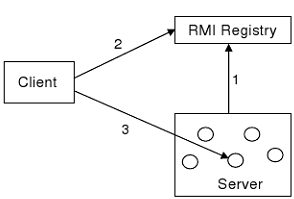
\includegraphics[scale=0.8]{Figurer/RMI-registry.png}
\caption{The use of the RMI Registry \cite{RMI-slides}}
\end{figure}
The registry is used to locate the remote object a Client need to use as it provides a name to a remote object's skeleton. Ones a remote object is registered on a server (1), clients can look up the objects by names (2) and obtain a remote object reference which is used to communicate with the wanted server and its remote object (3). Thus the registry provides the stub and the reference to the remote object \cite{Getting-started}.

\item The \textbf{Transport Layer} handles how the data is transported via the TCP/IP connection through a network. It is responsible for accepting calls on incoming connections, setting up the connection between JVM's and dispatch to the remote reference layer. It contains the following features:
\begin{itemize}
\item \textbf{Endpoint} used to denote the addresses to the client and the server; the address space or a JVM
\item \textbf{Channel} is responsible for managing the connection between the client and the server
\item \textbf{Connection} is used to transfer the data
\item \textbf{Transport}. Within a transport between a server and a client only one channel exist.
\end{itemize}

\setlength\parindent{300pt}\cite{RMI-slides}

\end{itemize}

MIA: Se evt. http://www.sce.carleton.ca/netmanage/simulator/rmi/RMIExplanation.htm og forklar RRL og Transport-layer bedre.

\section{Leader election}
When developing distributed systems there is multiple nodes(PC's) where there is running multiple processes. These processes cooperate to solving a given task. To control all these processes and secure the cooperation in solving the given task, it is important to elect a leader/coordinator, which all processes can interact with. To choose the given leader, the algoritm "Leader Election" is used.  The objective in leader election is that all process agrees on a leader and any process can serve as a leader and call an election. \cite{RMI-slides}. A leader election is used in the following scenarios
\begin{itemize}
\item When the system is initialized
\item When a leader fails
\item When a leader retires on purpose
\end{itemize}
To choose the leader, the network nodes communicate among themselves in order to decide which of them get the leader state. In order to archieve this, the different processes have to be unique and to have comparable identies, so they can compare between each other. When comparing, the leader node is the one with the highest identity/process number. \cite{wiki-Leader}. A simple example with one process per machine, the identity could be the mac adress of each machine.\cite{ElectionAlgorithm}
To locate the process with the highest number there is different leader election algoritms which will be explained in a later section. \\

When using leader election algorithms, everytime there is a election it cost on the hardware front, e.g. CPU, RAM, bandwith, battery, etc.\cite{RMI-slides} This can in worst case result in overload and a given process could fail e.g. due to hardware failure. The given process could be the leader and the algoritm would then take care of electing a new leader instead of the broken/failed process. This minimize the computational burden when using leader election. Furthermore it also take care of the others process can go on with a new leader and that they would work without the broken process, since there still is a leader which all processes can interact with.  \\

An example of a concrete leader election algorithm, could be the Bully election algorithm. Its mode of operation is when a given process notices that the leader/coordinator is no longer responding to requests and a given process then initiates an election. A process, P,  holds an election the following way
\begin{enumerate}
\item P sends an ELECTION message to all process with higher numbers
\item If no one responds, P wins the election and becomes leader/coordinator
\item If one of the higher ups processes answers, it takes over and P's jobs is done 
\end{enumerate}

The highest numbered running process will always win, which is charcterized as the "biggest guy in town", and hence the name "Bully algorithm".\cite{ElectionAlgorithm} There is always only one coordinator when using this algorithm. An concrete example of a bully algorithm can be explained as followed

\begin{figure}[hbtp]
\centering
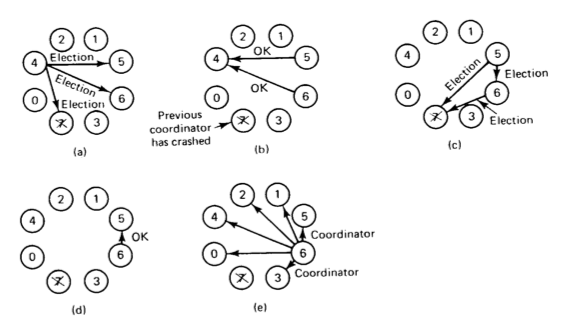
\includegraphics[scale=0.8]{Figurer/BullyAlgorithm.png}
\caption{Concrete example of Bully Algorithm}
\end{figure}

Some of the assumptions in the given example is that e.g. each process knows which processes have higher ID's and that each process can inter-communicate. \cite{RMI-slides} 

\begin{enumerate}[a)]
\item Process 7 was the coordinator but have crashed, and process 4 is the first one to notice. It sends an ELECTION message to all process above it, namely process 5,6 and 7.  
\item Process 5,6 which are running, returns a ANSWER message (OK) to process 4. 
\item When process 4 gets a OK from both 5 and 6, it will know its own job is done. Process 5 and 6 holds an election to the higher numbered processes. 
\item Process 6 returns an OK to process 5 and at this point it know that it will take over due to the fact that process 7 is crashed. 
\item Process 6 is the new leader and sends an COORDINATOR message(message with ID of the new coordinator) to all processes. This means that process 4 can now continue with the operation it was trying to handle, when process 7 didnt respond, now it is just using process 6 instead and the work can continue. 
\end{enumerate}

If process 7 will run again, it will send all the other running a COORDINATOR message and bully all the other processes into submission, and then again be leader/coordinator. \cite{ElectionAlgorithm} 

Another example of an algorithm, could be The Chang and Roberts algorithm, which is a ring-based coordinator election algorithm. The algorithm assumes that each process have a UID(Unique Identification) and that the processes can arrange themselves in a unidirectional ring with a communication channel going from each process to the clockweise neighbour.

When there is an election the given process sends its own ID(UID) as the ELECTION message, and passes it along. When a node recieves an id, it passes it along if its own ID is less than the id it received. When a node receives its own id, it set itself to be the leader. \cite{wiki-RingAlgorithm}


\end{document}  